\chapter{روش های پیشنهادی}



\subsection*{استفاده از روش‌های تانسوری در شبکه‌های عصبی چندلایه}

در سال‌های اخیر، استفاده از روش‌های تانسوری به‌عنوان روشی نوین در بهینه‌سازی معماری‌های شبکه‌های عصبی، به‌ویژه در مدل‌هایی که تعداد پارامترهای آن‌ها بسیار زیاد است، مانند شبکه‌های عصبی چندلایه \footnote{\lr{Mlp}}، توجه بسیاری را به خود جلب کرده است \cite{novikov2015tensorizing}. تانسورها تعمیمی از ماتریس‌ها به ابعاد بالاتر هستند و به‌طور طبیعی برای نمایش داده‌های چندبعدی همچون تصاویر، ویدیوها یا سری‌های زمانی چندکاناله مناسب‌اند. بهره‌گیری از ساختار تانسوری در معماری شبکه، این امکان را فراهم می‌سازد که بدون نیاز به فشرده‌سازی اولیه (مانند صاف کردن \footnote{\lr{flatten}} کردن ورودی)، اطلاعات ساختاری میان ابعاد مختلف حفظ شده و مدل بتواند از روابط درون‌تعاملی موجود میان این ابعاد بهره‌برداری نماید \cite{novikov2015tensorizing}.

در معماری سنتی شبکه عصبی چند لایه، نگاشت از ورودی \lr{$\mathbf{x} \in \mathbb{R}^n$} به خروجی \lr{$\mathbf{y} \in \mathbb{R}^m$} به‌وسیله ضرب ماتریسی انجام می‌گیرد:

\[
\mathbf{y} = W\mathbf{x} + \mathbf{b}
\]

که در آن \lr{$W \in \mathbb{R}^{m \times n}$} ماتریس وزن و \lr{$\mathbf{b}$} بردار بایاس است.

\begin{figure}[h]
	\centering
	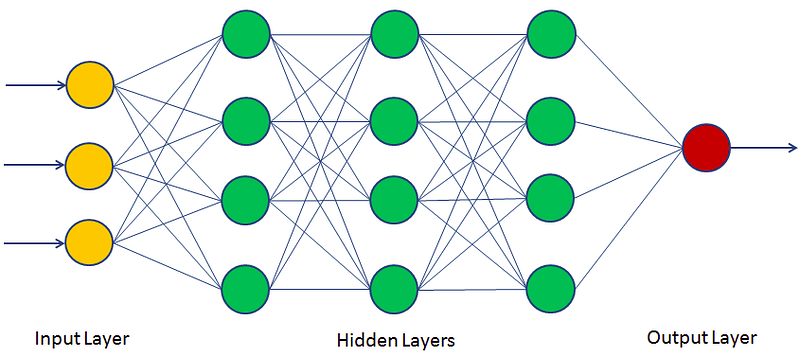
\includegraphics[width=0.8\textwidth]{transformer_images/mlp.png}
	\caption{شبکه عصبی پرسپترون چند لایه}
	\label{fig:Mlp}
\end{figure}

در مقابل، در روش‌های تانسوری، وزن‌ها به‌صورت یک تانسور مرتبه بالاتر مدل‌سازی می‌شوند و نگاشت ورودی به خروجی با استفاده از ضرب‌های چندحالته (ضرب تانسوری در ابعاد مختلف) صورت می‌پذیرد:

\[
\mathbf{y} = \mathcal{W} \times_1 \mathbf{x}_1 \times_2 \mathbf{x}_2 \times_3 \cdots + \mathbf{b}
\]

در این رابطه، \lr{$\mathcal{W}$} یک تانسور وزن است و عملگر \lr{$\times_n$} نشان‌دهنده ضرب تانسوری در بعد $n$‌ام می‌باشد.

روش‌هایی نظیر \lr{TCL} \footnote{tensor contraction layer} و \lr{TRL} \footnote{Tensor regression layer} به‌عنوان نمونه‌هایی از این رویکرد، با بهره‌گیری از تکنیک‌های تجزیه تانسوری همچون \lr{Tucker} یا تجزیه \lr{CP}، نه تنها باعث کاهش چشمگیر در تعداد پارامترها می‌شوند، بلکه ساختار چندبعدی داده‌ها را نیز حفظ می‌نمایند \cite{kossaifi2017tensorcontraction, kossaifi2020tensorregression}.

\subsection*{مزایای استفاده از روش‌های تانسوری}

استفاده از روش‌های تانسوری در شبکه‌های عصبی چندلایه مزایای متعددی به همراه دارد که برخی از مهم‌ترین آن‌ها عبارت‌اند از:

\begin{itemize}
	\item \textbf{کاهش چشمگیر تعداد پارامترها:} با بهره‌گیری از فشرده‌سازی تانسوری، می‌توان ابعاد تانسور وزن‌ها را به‌گونه‌ای کاهش داد که بدون افت محسوس در عملکرد مدل، مصرف حافظه و پیچیدگی محاسباتی به‌طور قابل توجهی کاهش یابد \cite{lebedev2015cp, kossaifi2020tensorregression}.
	
	\item \textbf{حفظ ساختار داده‌های ورودی:} برخلاف روش‌های سنتی که در آن‌ها داده‌ها پیش از ورود به لایه‌های چگال \footnote{\lr{Dense}} باید مسطح‌سازی \footnote{\lr{Flatten}} شوند، استفاده از ساختار تانسوری این امکان را فراهم می‌کند که ساختار فضایی، زمانی یا کانالی داده‌ها حفظ شده و ارتباط میان ابعاد مختلف ورودی بهتر درک و پردازش شود \cite{kossaifi2020tensorregression}.
\end{itemize}

\subsection*{محدودیت‌ها و چالش‌ها}

با وجود مزایای متعدد، بهره‌گیری از روش‌های تانسوری در معماری‌های شبکه‌های عصبی با چالش‌ها و محدودیت‌هایی نیز همراه است که در ادامه به برخی از مهم‌ترین آن‌ها اشاره می‌شود:

\begin{itemize}
	\item \textbf{پیچیدگی بالاتر در پیاده‌سازی:} پیاده‌سازی لایه‌های مبتنی بر عملیات تانسوری معمولاً به ابزارها و کتابخانه‌های خاصی همچون \lr{Tensorly} یا \lr{Tensor Toolbox} نیاز دارد. این موضوع فرآیند طراحی و توسعه مدل را پیچیده‌تر از استفاده از لایه‌های استاندارد مانند شبکه عصبی چند لایه می‌سازد \cite{kossaifi2017tensorcontraction}.
	
	\item \textbf{بهینه‌سازی دشوارتر:} فرآیند آموزش مدل‌های تانسوری می‌تواند نسبت به مدل‌های معمولی کندتر باشد. الگوریتم‌های مبتنی بر گرادیان ممکن است در فضای پارامتری تانسورها با سطوح خطای غیرهموار یا چندوجهی مواجه شوند که روند همگرایی را دشوار می‌کند \cite{yang2017ttrnn}.
	
	\item \textbf{احتمال کاهش دقت در فشرده‌سازی شدید:} در صورتی‌که میزان فشرده‌سازی تانسورها بیش از حد بالا باشد، مدل ممکن است توانایی لازم برای نمایش روابط غیرخطی و الگوهای پیچیده را از دست داده و در نتیجه، دقت نهایی پیش‌بینی کاهش یابد \cite{kossaifi2020tensorregression}.
\end{itemize}



\subsection{لایه فشرده‌سازی تانسوری}


\lr{Tensor Contraction Layer}

در بسیاری از مدل‌های یادگیری عمیق—به‌ویژه شبکه‌های عصبی کانولوشنی (\lr{convolution})—فعال‌سازی‌های لایه‌های میانی به‌شکل تانسورهایی با مرتبه بالا ظاهر می‌شوند. به‌طور سنتی، برای اعمال لایه‌های کاملاً متصل (\lr{Fully Connected})، این تانسورها ابتدا با عملیات مسطح‌سازی (\lr{flatten}) به بردار تبدیل و سپس به فضای خروجی نگاشت می‌شوند؛ روشی که ساختار چندخطی (\lr{multilinear structure}) داده را از بین برده و به‌تبع، تعداد پارامترها افسارگسیخته افزایش می‌یابد \cite{kossaifi2020tensorregression}.

در پاسخ به این چالش، لایه‌ای با عنوان **­لایهٔ فشرده‌سازی تانسوری** یا به اختصار \lr{TCL} معرفی شده است. این لایه بدون نیاز به مسطح‌سازی، هر مد (mode) از تانسور ورودی را مستقل فشرده‌سازی می‌کند و ساختار چندخطی داده را حفظ می‌نماید \cite{kossaifi2017tensorcontraction,kossaifi2020tensorregression}.



\begin{figure}[h]
	\centering
	\begin{minipage}[b]{0.7\textwidth}
		\centering
		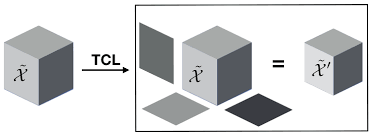
\includegraphics[width=\textwidth]{transformer_images/tcl.png}
		\caption{لایه فشرده ساز تانسوری}
		\label{fig:tensor_contraction_layer}
	\end{minipage}
	\hfill
\end{figure}




\subsubsection*{فرمول‌بندی ریاضی}

فرض کنید تانسور فعال‌سازی ورودی:
\[
\mathcal{X} \in \mathbb{R}^{S \times I_0 \times I_1 \times \cdots \times I_N}
\]
باشد (که \(S\) اندازهٔ دسته‌بندی و \(I_k\)ها ابعاد کانال/فضایی را نشان می‌دهند). هدف لایه TCL، نگاشت:
\[
\mathcal{X}' = \mathcal{X} \times_1 V^{(0)} \times_2 V^{(1)} \cdots \times_{N+1} V^{(N)}
\]
است، که در آن:
\[
V^{(k)} \in \mathbb{R}^{R_k \times I_k}, \quad \forall k = 0,\dots,N.
\]
با این عملگرهای ضرب چندحالته (\(\times_n\)) تعداد پارامترها به‌شکلی چشمگیر کاهش می‌یابند \cite{kossaifi2017tensorcontraction}.







\subsubsection*{تحلیل تعداد پارامترها}

در TCL، کل پارامترهای قابل آموزش برابر است با:
\[
\text{پارامترهای TCL} = \sum_{k=0}^{N} I_k \cdot R_k
\]
در حالی‌که در لایه متصل سنتی (پس از مسطح‌سازی):
\[
\text{پارامترهای FC} = \left(\prod_{k=0}^{N} I_k\right) \cdot O
\]
که \(O\) تعداد نورون‌های خروجی لایه است. نمایش ریاضی بالا به‌وضوح نشان می‌دهد که TCL با جایگزینی ضرب با جمع ساده، به‌صرفه‌سازی قابل‌توجهی در حافظه و محاسبات مدل منجر می‌شود \cite{kossaifi2017tensorcontraction,kossaifi2020tensorregression}.

\subsection{لایهٔ رگرسیون تانسوری (\lr{TRL})}

این لایه، خروجی مدل را مستقیماً از تانسور ورودی تولید می‌کند، بدون مسطح‌سازی؛ به‌طوری‌که ساختار چندبعدی ورودی حفظ و نگاشت خروجی نیز به‌صورت مرتبۀ پایین (low‑rank) مدل شده است \cite{kossaifi2020tensorregression}.

\subsubsection*{فرمول‌بندی ریاضی}

فرض مجدد تانسور:
\[
\mathcal{X} \in \mathbb{R}^{S \times I_0 \times I_1 \times \cdots \times I_N}
\]
و تانسور وزن:
\[
\mathcal{W} \in \mathbb{R}^{I_0 \times I_1 \times \cdots \times I_N \times O}.
\]
نگاشت خروجی:
\[
\mathbf{Y} = \langle \mathcal{X}, \mathcal{W} \rangle_N + \mathbf{b}
\]
در اینجا عملگر \(\langle \cdot,\cdot \rangle_N\) ضرب داخلی روی \(N\) بعد اول \(\mathcal{W}\) و \(N\) بعد اول \(\mathcal{X}\) را نشان می‌دهد \cite{kossaifi2020tensorregression}.

برای کاهش پارامترها، \(\mathcal{W}\)‌ با کمک تجزیۀ توکر به شکل زیر نوشته می‌شود:
\[
\mathcal{W} = \mathcal{G} \times_0 U^{(0)} \times_1 U^{(1)} \cdots \times_N U^{(N)} \times_{N+1} U^{(N+1)},
\]
که \(\mathcal{G}\) هستهٔ کم‌مرتبه (core tensor) و \(U^{(k)}\) ماتریس‌های فشرده‌سازی هستند \cite{kossaifi2020tensorregression}.

فرمول نهایی:
\[
\mathbf{Y} = \left\langle \mathcal{X} \times_0 (U^{(0)})^\top \cdots \times_N (U^{(N)})^\top, \mathcal{G} \times_{N+1} U^{(N+1)} \right\rangle_N + \mathbf{b}
\]
که به‌صورت محاسباتی بهینه‌تر عمل می‌کند \cite{kossaifi2020tensorregression}.

\subsubsection*{تحلیل تعداد پارامترها}

در لایه TRL با تجزیۀ \(\text{Tucker}\)، تعداد پارامترها برابر است با:
\[
\text{پارامترهای TRL} = \left(\prod_{k=0}^{N+1} R_k\right) + \left(\sum_{k=0}^{N} I_k R_k\right) + R_{N+1} \cdot O,
\]
که معمولاً بسیار کمتر از تعداد پارامترهای لایه FC است، به‌ویژه هنگامی که \(R_k \ll I_k\) انتخاب شوند \cite{kossaifi2020tensorregression}.


\subsection{چرا در مبدل‌های بینایی از تانسور استفاده می‌کنیم؟}

\subsubsection{۱. \textbf{کاهش تعداد پارامترها و حافظه مصرفی}}

یکی از چالش‌های اصلی در معماری‌های مبتنی بر مبدل‌های بینایی، رشد نمایی تعداد پارامترها در لایه‌های کاملاً متصل، به‌ویژه در بخش‌های انتهایی شبکه است. با جایگزینی این لایه‌ها با ساختارهای تانسوری مانند TCL و TRL، می‌توان از ساختار چندبعدی داده بهره برده و از طریق تجزیه‌های کم‌مرتبه، تعداد پارامترها را به‌صورت چشمگیری کاهش داد \cite{novikov2015tensorizing, kossaifi2017tensorcontraction, kossaifi2020tensorregression}. این جایگزینی نه‌تنها موجب صرفه‌جویی در حافظه می‌شود، بلکه پیچیدگی محاسباتی مدل را نیز کاهش داده و امکان به‌کارگیری آن را در محیط‌های کم‌منبع (مانند دستگاه‌های لبه‌ای و موبایل) فراهم می‌سازد \cite{hamreras2025tensorization}.

\subsubsection{۲. \textbf{افزایش تفسیرپذیری با حفظ ساختار چندخطی داده}}

در حالی‌که عملیات مسطح‌سازی بر روی تانسورهای ورودی، ساختار ارتباطی میان ابعاد داده را از بین می‌برد، استفاده از لایه‌های تانسوری (TCL و TRL) این ساختار چندخطی را حفظ می‌کند. این امر نه‌تنها مدل را برای کار با داده‌های فضایی یا زمانی چندکاناله مطلوب‌تر می‌سازد بلکه \emph{قابلیت تفسیرپذیری پیش‌بینی‌های مدل} را نیز ارتقا می‌دهد. چرا که استحصال ساختارهای فیچر درون تانسوری (مثلاً بعدهای اساسی کابل‌ها) می‌تواند به تشریح بهتر مسیرهای تصمیم‌گیری مدل کمک کند \cite{hamreras2025tensorization}.

\subsubsection{۳. \textbf{کاهش نیاز به داده‌های آموزشی بزرگ}}

مدل‌های بینایی مبتنی بر مبدل، به‌دلیل فقدان سوگیری‌های مکانی ذاتی شبکه‌های کانولوشنی، نیازمند حجم عظیمی از داده برای آموزش مؤثر هستند. با استفاده از لایه‌های تانسوری مانند TCL و TRL که نگاشت‌ها را به‌صورت چندخطی و فشرده مدل‌سازی می‌کنند و ساختار درونی داده را حفظ می‌کنند، می‌توان از ظرفیت مدل به‌صورت بهینه‌تر بهره برد. این ساختار نه‌تنها کمک می‌کند وابستگی‌های میان‌بُعدی بهتر درک شوند بلکه از بیش‌برازش در شرایط داده‌ی محدود جلوگیری می‌کند؛ به‌عنوان مثال، در روش FacT (Factor‑Tuning)، فقط \(0.01\%\) پارامترهای ViT برای تعداد بسیار کمی از نمونه‌های آموزشی آموزش داده می‌شود و با صرفه‌جویی قابل‌توجه در پارامترها، عملکردی مشابه یا بهتر از تنظیم کامل (full‑tuning) ارائه می‌دهد \cite{jie2022fact}.


\subsection{روش تانسوری مبدل پنجره متحرک:}




\subsection{پیاده‌سازی مرحله‌ی  تعبیه پچ
	با استفاده از فشرده‌سازی تانسوری}

در معماری‌های کلاسیک مبتنی بر مبدل های بیانی \footnote{\lr{Vision transformer}}  و همچنین در ساختار مبدل های پنجره ای \footnote{\lr{swin transformer}}، مرحله‌ی اولیه‌ی پردازش تصویر شامل تقسیم تصویر به قطعات کوچک (پچ‌ها) و سپس نگاشت هر پچ به یک بردار نهفته با ابعاد ثابت است. این نگاشت معمولاً با استفاده از یک لایه‌ی خطی \footnote{\lr{linear}} یا پیچشی \footnote{\lr{convolution}} با کرنل و گام برابر با اندازه‌ی پچ انجام می‌شود.

در روش تانسوری به‌جای استفاده از نگاشت برداری ساده، از لایه‌ی فشرده‌سازی تانسوری \footnote{\lr{tensor contruction layer}} برای تبدیل هر پچ به یک تانسور چندبعدی در فضای ویژگی استفاده شده است. این نگاشت تانسوری نه‌تنها باعث حفظ ساختار چندخطی پچ‌ها می‌شود، بلکه با فشرده‌سازی موثر، منجر به کاهش پارامترها می شود.




در ابتدا فرض میکنیم  ورودی مدل تصویری با اندازه‌ی \lr{$(B, C, H, W)$} باشد که در آن:

\begin{itemize}
	\item $B$ اندازه‌ی دسته‌ی آموزشی \footnote{\lr{Batch Size}} است.
	\item $C$ تعداد کانال‌های تصویر (برای مثال ۳ در تصاویر رنگی).
	\item $H \times W$ ابعاد تصویر است.
\end{itemize}

این تصویر با استفاده از پچ‌هایی با اندازه‌ی \lr{$(P \times P)$} به $\frac{H}{P} \times \frac{W}{P}$ قطعه تقسیم می‌شود. سپس با استفاده از عملیات بازآرایی \footnote{\lr{rearrangement}}، ساختار ورودی به شکل زیر تبدیل می‌شود:

\[
\mathcal{X} \in \mathbb{R}^{B \times P_1 \times P_2 \times C_1 \times C_2 \times C_3}
\]

که در آن:

\begin{itemize}
	\item $P_1 = \frac{H}{P}$ و $P_2 = \frac{W}{P}$ به‌ترتیب تعداد پچ‌ها در راستای ارتفاع و عرض تصویر هستند.
	\item $C_1 = P$ و $C_2 = P$ ابعاد مکانی هر پچ‌اند.
	\item $C_3 = C$ تعداد کانال‌های تصویر ورودی است.
\end{itemize}

در این بازنمایی، هر پچ در موقعیت $(i,j)$ به‌صورت یک تانسور سه‌بعدی با ابعاد $C_1 \times C_2 \times C_3$ نمایش داده می‌شود. این ساختار چندبعدی امکان استفاده‌ی مستقیم از عملیات تانسوری بدون نیاز به تخت‌سازی را فراهم می‌سازد.



برای نگاشت هر پچ به فضای نهفته، به جای استفاده از mlp  از یک لایه‌ی فشرده ساز تانسوری  استفاده می‌شود. در واقع سه تا بعد اخر با استفاده از لایه فشرده ساز تنسوری تعبیه میشود.

\[
\mathcal{Z} \in \mathbb{R}^{B \times P_1 \times P_2 \times D_1 \times D_2 \times D_3}
\]

در این ساختار، هر پچ به‌جای تبدیل به یک بردار تخت، به یک تانسور سه‌بعدی در فضای نهفته تبدیل می‌شود. این تانسور ساختار درونی پچ را حفظ کرد می کند. 

\subsubsection*{فرمول‌بندی ریاضی عملیات فشرده‌سازی}

فرض میکنیم  $\mathcal{X}_{patch} \in \mathbb{R}^{C_1 \times C_2 \times C_3}$ نمایانگر یک پچ ورودی باشد. برای فشرده‌سازی این تانسور به فضای نهفته $(D_1, D_2, D_3)$، از سه ماتریس فشرده‌سازی قابل آموزش استفاده می‌شود:

\[
V^{(0)} \in \mathbb{R}^{D_1 \times C_1}, \quad
V^{(1)} \in \mathbb{R}^{D_2 \times C_2}, \quad
V^{(2)} \in \mathbb{R}^{D_3 \times C_3}
\]

عملیات فشرده‌سازی با استفاده از ضرب‌های چندحالته \footnote{\lr{n-mode product}} صورت می‌گیرد:

\[
\mathcal{X}_{emb} = \mathcal{X}_{patch} \times_0 V^{(0)} \times_1 V^{(1)} \times_2 V^{(2)}
\]

که در آن $\mathcal{X}_{emb} \in \mathbb{R}^{D_1 \times D_2 \times D_3}$ نگاشت نهفته‌ی تانسوری برای آن پچ خواهد بود.

در این مدل ساختار چند بعدی به پج ها داده میشود و همچنین با استفاده از تانسور تعداد پارامتر ها کاهش پیدا میکنند و همچنین ظرفیت مدل نیز افزایش پیدا میکند.




در نتیجه، خروجی نهایی مرحله‌ی تعبیه پچ به‌صورت زیر تعریف می‌شود:

\[
\mathcal{Z} \in \mathbb{R}^{B \times P_1 \times P_2 \times D_1 \times D_2 \times D_3}
\]

که در آن هر پچ به‌صورت یک تانسور کم‌بعد در فضای نهفته نمایش داده شده است.


\subsection{ماژول توجه سلف چندسری مبتنی بر پنجره به‌صورت تانسوری}

همانطور که در فصل قبل بیان شد در ساختار مبدل پنجره ای، جهت کاهش پیچیدگی محاسباتی، از روشی با عنوان  \footnote{\lr{Window-based Multi-Head Self-Attention}}بهره گرفته می‌شود. در این روش، ویژگی‌های مکانی تصویر به پنجره‌های کوچک با اندازه‌ی ثابت (بدون هم‌پوشانی) تقسیم شده و سپس عملیات  خود‌توجهی به‌صورت محلی و درون هر پنجره مستقل انجام می‌گیرد.

در روش تانسوری، به‌جای تولید بردارهای تخت‌شده‌ی $Q$، $K$ و $V$، این بردارها به‌صورت \textbf{تانسورهای چندبعدی} با استفاده از لایه فشرده ساز تانسوری تولید می‌شوند.

\subsubsection*{ ساختار ورودی و تقسیم به پنجره‌ها}

خروجی مرحله تعبیه  به‌صورت تانسوری به صورت زیر است 

\[
\mathcal{X} \in \mathbb{R}^{B \times H \times W \times D_1 \times D_2 \times D_3}
\]



در گام اول، همانند مبدل های پنجره ای به پنجره‌های $w \times w$ تقسیم می‌شوند. و خروجی ما به صورت  زیر خواهد بود.

\[
\mathcal{X}_{win} \in \mathbb{R}^{B \times N_H \times N_W \times w \times w \times D_1 \times D_2 \times D_3}
\]

که در آن $N_H = \frac{H}{w}$ و $N_W = \frac{W}{w}$ به‌ترتیب تعداد پنجره‌ها در راستای ارتفاع و عرض تصویر هستند.

\subsubsection*{2. محاسبه‌ی Q، K و V با استفاده از لایه فشرده ساز تانسوری}

برای هر پنجره‌ی مکانی، سه لایه‌ی فشرده‌سازی تانسوری مستقل (\lr{TCL}) برای استخراج تانسورهای Q، K و V طراحی شده‌اند. فرض می‌شود تانسور ورودی هر پنجره دارای ابعاد:

\[
\mathcal{X}_{patch} \in \mathbb{R}^{w \times w \times D_1 \times D_2 \times D_3}
\]

باشد. با اعمال سه عملیات ضرب n-مد به‌ترتیب در ابعاد تانسوری، نگاشت‌های Q، K و V به‌صورت زیر حاصل می‌شوند:

\[
\mathcal{Q} = \mathcal{X}_{patch} \times_2 V_Q^{(1)} \times_3 V_Q^{(2)} \times_4 V_Q^{(3)}
\]
\[
\mathcal{K} = \mathcal{X}_{patch} \times_2 V_K^{(1)} \times_3 V_K^{(2)} \times_4 V_K^{(3)}
\]
\[
\mathcal{V} = \mathcal{X}_{patch} \times_2 V_V^{(1)} \times_3 V_V^{(2)} \times_4 V_V^{(3)}
\]

که در آن هر $V^{(i)}$ ماتریس فشرده‌سازی با ابعاد $\mathbb{R}^{D_i \times D_i}$ است. بنابراین، خروجی هر لایه به فضای تانسوری مشابه با ورودی بازمی‌گردد:

\[
\mathcal{Q}, \mathcal{K}, \mathcal{V} \in \mathbb{R}^{w \times w \times D_1 \times D_2 \times D_3}
\]

\subsubsection*{3. تقسیم سرهای توجه چندگانه}

برای پیاده‌سازی مکانیزم چندسر\footnote{\lr{multi-head}}، ابعاد تانسوری خروجی به بخش‌های کوچک‌تری تقسیم می‌شود. فرض می‌شود:

\[
D_1 = h_1 \cdot d_1, \quad D_2 = h_2 \cdot d_2, \quad D_3 = h_3 \cdot d_3
\]

که در آن:
\begin{itemize}
	\item $h_1, h_2, h_3$ تعداد سرها در هر بُعد تانسوری،
	\item $d_1, d_2, d_3$ ابعاد نهفته‌ی هر سر در هر بُعد هستند.
\end{itemize}

با استفاده از عملیات بازآرایی، تانسورهای Q، K و V به شکل زیر سازمان‌دهی می‌شوند:

\[
\mathcal{Q}_{head} \in \mathbb{R}^{B \times N_H \times N_W \times w \times w \times h_1 \times h_2 \times h_3 \times d_1 \times d_2 \times d_3}
\]

و ساختار مشابهی برای K و V در نظر گرفته می‌شود.

\subsubsection*{4. محاسبه ماتریس توجه تانسوری}

عملیات ضرب داخلی تعمیم‌یافته بین تانسورهای Q و K برای محاسبه‌ی ماتریس توجه انجام می‌شود. برای هر سر $(a,b,c)$ و برای موقعیت‌های $(i,j)$ و $(k,l)$ در پنجره، مقدار توجه به‌صورت زیر محاسبه می‌شود:

\[
\text{Attention}_{ijkl}^{abc} = \sum_{x=1}^{d_1} \sum_{y=1}^{d_2} \sum_{z=1}^{d_3} Q_{ij}^{abcxyz} \cdot K_{kl}^{abcxyz}
\]

که نتیجه نهایی یک ماتریس توجه با ابعاد زیر است:

\[
\text{Attention} \in \mathbb{R}^{B \times N_H \times N_W \times h_1 \times h_2 \times h_3 \times w^2 \times w^2}
\]

برای پایدارسازی محاسبات، نرمال‌سازی زیر اعمال می‌شود:

\[
\text{scale} = \frac{1}{\sqrt{d_1 d_2 d_3}}
\]

و از نسخه علامت‌دار تابع softmax برای اعمال توجه استفاده می‌گردد:

\[
\text{Attention}_{\text{soft}} = \text{sign}(A) \cdot \text{softmax}(|A|)
\]

\subsubsection*{5. اعمال توجه و بازسازی ویژگی}

پس از محاسبه ماتریس توجه، تانسور خروجی هر پنجره با استفاده از ترکیب توجه و تانسور V محاسبه می‌شود:

\[
\mathcal{Y}_{ij}^{abcxyz} = \sum_{k,l} \text{Attention}_{ijkl}^{abc} \cdot V_{kl}^{abcxyz}
\]

و پس از انجام توجه برای هر پنجره دوباره باز آرایی میشوند و به حالت اولیه باز میگردند و ابعاد آن به صورت زیر میشود.

\[
\mathcal{Y} \in \mathbb{R}^{B \times H \times W \times D_1 \times D_2 \times D_3}
\]

در این مدل چون سر ها در سه بعد تفسیم میشوند در نتیجه این مدل آزادی خیلی بیشتری دارد.






\subsection{توجه علامت‌دار}

در مکانیزم‌های استاندارد خود توجهی که در مبدل ها مورد استفاده قرار می‌گیرند، ماتریس‌های $Q$, $K$ و $V$ با یکدیگر تعامل دارند تا وزن‌های توجه استخراج شوند. در این فرآیند، بردارهای $Q$  \footnote{\lr{Query}}
 و $K$ 
 
 \footnote{\lr{Key}}
  با استفاده از ضرب داخلی محاسبه می‌شوند و نتیجه برای هر توکن، بیان‌گر میزان اهمیت نسبی سایر توکن‌ها در ارتباط با آن توکن است.

فرمول رایج محاسبه توجه به‌صورت زیر تعریف می‌شود:

\[
\text{Attention}(Q, K, V) = \text{Softmax}\left( \frac{QK^\top}{\sqrt{d_k}} \right) V
\]

در این ساختار، خروجی $QK^\top$ می‌تواند شامل مقادیر مثبت، منفی یا صفر باشد؛ اما پس از اعمال تابع \lr{Softmax}، تمامی مقادیر به‌صورت نرمال‌سازی‌شده و مثبت خواهند بود. در نتیجه،اطلاعات قطبیت (علامت) که در نتیجه‌ی ضرب داخلی بین بردارهای $Q$ و $K$ وجود داشت، از بین می‌رود. این ویژگی باعث محدود شدن ظرفیت مدل در شناسایی «رابطه منفی یا متضاد» میان توکن‌ها می‌شود.

برای حفظ این اطلاعات قطبیت، د از رویکردی با عنوان  توجه علامت دار استفاده شده است. ایده‌ی اصلی این روش آن است که پس از محاسبه‌ی امتیازهای توجه $A = QK^\top$، عملیات نرمال‌سازی \lr{Softmax} بر قدرمطلق این امتیازها انجام شده و سپس علامت اولیه آن‌ها به نتیجه بازگردانده می‌شود.

فرمول این روش به‌صورت زیر تعریف می‌شود:

\[
\text{Attention}_{\text{sign}} = \text{sign}(A) \cdot \text{Softmax}(|A|)
\]

که در آن:
\begin{itemize}
	\item $A = QK^\top$ ماتریس امتیازهای اولیه توجه است.
	\item $\text{sign}(A)$ عملیاتی است که علامت هر مقدار را حفظ می‌کند (مقادیر $+1$, $-1$ یا $0$).
	\item $|A|$ قدرمطلق مقادیر است که شدت شباهت را بدون در نظر گرفتن جهت نشان می‌دهد.
\end{itemize}


برای درک بهتر تفاوت میان مکانیزم‌های توجه معمولی و توجه علامت دار یک مثال عددی ساده اما گویای زیر ارائه می‌شود.

فرض کنیم  بردار پرس‌وجو (Q) و دو بردار کلید (K) به‌صورت زیر تعریف شده‌اند:

\[
Q = [1,\ 2,\ -1], \quad
K_1 = [1,\ 0,\ -1], \quad
K_2 = [-1,\ 1,\ 1]
\]

\paragraph{محاسبه امتیاز توجه}

ابتدا شباهت میان Q و هر کلید با استفاده از ضرب داخلی محاسبه می‌شود:

\[
Q \cdot K_1 = (1)(1) + (2)(0) + (-1)(-1) = 1 + 0 + 1 = 2
\]
\[
Q \cdot K_2 = (1)(-1) + (2)(1) + (-1)(1) = -1 + 2 -1 = 0
\]

بنابراین بردار امتیاز توجه به‌صورت زیر حاصل می‌شود:

\[
A = [2,\ 0]
\]

\paragraph{الف) توجه معمولی:}

در توجه معمولی، از تابع softmax مستقیماً روی مقادیر $A$ استفاده می‌شود:

\[
\text{Softmax}(A) =
\left[
\frac{e^2}{e^2 + e^0},\ 
\frac{e^0}{e^2 + e^0}
\right]
\approx [0.88,\ 0.12]
\]

در اینجا، هر دو کلید مقدار وزن مثبت می‌گیرند، حتی اگر امتیاز شباهت دومی برابر با صفر بوده باشد. مدل نمی‌تواند تفاوت میان بی‌اثر بودن و تأثیر منفی یا متضاد را به‌خوبی درک کند.

\paragraph{ب) توجه علامت‌دار:}

در این رویکرد، ابتدا بردار $A$ به دو بخش علامت و قدرمطلق تفکیک می‌شود:

\[
\text{sign}(A) = [1,\ 0], \quad
|A| = [2,\ 0]
\]

سپس تابع softmax فقط روی قدرمطلق‌ها اعمال شده و خروجی زیر حاصل می‌شود:

\[
\text{Softmax}(|A|) = 
\left[
\frac{e^2}{e^2 + e^0},\ 
\frac{e^0}{e^2 + e^0}
\right]
\approx [0.88,\ 0.12]
\]

در نهایت، با ضرب عنصر‌به‌عنصر با علامت‌ها:

\[
\text{Attention}_{\text{sign}} = 
\text{sign}(A) \cdot \text{Softmax}(|A|) = [0.88,\ 0.00]
\]

در این حالت، کلید دوم به‌طور کامل کنار گذاشته شده است، چرا که امتیاز آن صفر بوده و نشانی از تأثیر مثبت یا منفی ندارد.


در توجه معمولی، تمامی مقادیر صفر یا منفی به وزن‌های مثبت نرمال‌سازی می‌شوند. در مقابل، توجه علامت‌دار توانایی تمایز بین ارتباط مثبت، منفی و خنثی را دارد. این قابلیت می‌تواند در مدل‌سازی دقیق‌تر تضادهای معنایی یا شباهت‌های منفی نقش مهمی ایفا کند.


\subsection{توجه مبتنی بر پنجره‌های جابه‌جا‌شده به صورت تانسوری}



توجه پنجره ای دارای یک محدودیت مهم است: پچ‌های واقع در پنجره‌های متفاوت هیچ‌گونه تبادل اطلاعاتی ندارند.
در حالی که ممکن هست این پج ها به هم نزدیک باشند به‌منظور رفع این محدودیت، مبدل های پنجره ای مکانیزم توجه مبتنی بر پنجره جا به جا شده معرفی شده است که در آن پنجره‌ها در برخی لایه‌ها به‌صورت جابه‌جا‌شده تعریف می‌شوند و از ماسک توجه برای جلوگیری از تداخل غیرمجاز استفاده می‌شود.

\subsubsection*{مراحل دقیق مکانیزم }

\begin{enumerate}
	\item \textbf{شیفت چرخشی تانسور ورودی:} خروجی مرحله قبلی  با یک  شیفت چرخه ای 
	\footnote{\lr{cyclic shift}} به اندازه $\lfloor \frac{w}{2} \rfloor$ پیکسل در راستای افقی و عمودی جابه‌جا می‌شود. این جابه‌جایی باعث می‌شود که پچ‌هایی که پیش‌تر در پنجره‌های جداگانه بودند، اکنون در یک پنجره جدید قرار گیرند.
	
	به این شیفت روی بعد اول و دوم تانسور که مکان پج را مشخص میکرد صورت میگیرد.
	
	\item \textbf{اعمال پنجره‌بندی جدید:} تانسور جابه‌جا‌شده به پنجره‌های بدون هم‌پوشانی جدید با اندازه $w \times w$ تقسیم می‌شود. پنجره‌های جدید از موقعیت‌های مختلف تصویر تشکیل شده‌اند.
	
	\item \textbf{اعمال خودتوجهی به‌صورت محلی با ماسک:} از آنجا که پنجره‌ها پس از شیفت ممکن است شامل توکن‌هایی از مکان‌های نامرتبط باشند، نیاز است که \textbf{توجه به‌صورت مفید  انجام شود. یک ماسک دودویی روی ماتریس توجه اعمال می‌شود که فقط اجازه توجه به توکن‌هایی را می‌دهد که واقعاً در یک پنجره معتبر قرار دارند.}
	
\end{enumerate}



خودتوجهی پنجره جابه جا شده باعث ارتباط میان پج های نزدیکی میشود که در خودتوجهی پنجره ای در یک پنجره قرار نداشته اند. 



\subsection{ادغام پچ‌ها به‌صورت تانسوری}

در مدل‌های سلسله‌مراتبی بینایی مانند پس از هر مرحله از استخراج ویژگی، لازم است ابعاد مکانی تصویر کاهش یابد تا ویژگی‌ها در سطوح بالاتر به‌صورت فشرده‌تر و معنایی‌تر نمایش داده شوند. این فرایند با عنوان ادغام پچ‌ها \footnote{\lr{Patch Merging}} شناخته می‌شود. در نسخه‌ی اصلی این مدل، ادغام پچ‌ها با استفاده از ترکیب ۴ پچ مجاور (به‌صورت یک پنجره‌ی $2 \times 2$) و سپس اعمال یک لایه‌ی خطی پس از مسطح‌سازی انجام می‌شود. این کار باعث نصف شدن ابعاد مکانی و افزایش ابعاد ویژگی می‌شود.

در این پژوهش، رویکرد متفاوتی برای ادغام پچ‌ها ارائه شده است که مبتنی بر نگاشت تانسوری است. به‌جای انجام \footnote{\lr{flatten}} بر روی پچ‌ها، از ساختار چندبعدی پچ‌ها استفاده شده و با کمک یک لایه‌ی فشرده‌سازی تانسوری، ادغام پچ‌ها بدون از بین رفتن ساختار چندخطی آن‌ها انجام می‌شود.

\subsubsection*{ساختار ورودی}

مانند  خروجی مرحله قبلی شبکه دارای ساختار تانسوری زیر باشد:

\[
\mathcal{X} \in \mathbb{R}^{B \times H \times W \times R_1 \times R_2 \times C}
\]

که در آن:

\begin{itemize}
	\item $B$ اندازه دسته آموزشی،  
	\item $H \times W$ ابعاد مکانی پچ‌ها،  
	\item $(R_1, R_2, C)$ ابعاد فضای نهفته‌ی هر پچ به‌صورت تانسوری.
\end{itemize}

هدف این مرحله، کاهش ابعاد مکانی به $\left( \frac{H}{2}, \frac{W}{2} \right)$ و در عین حال، افزایش غنای بازنمایی ویژگی‌ها است.

\subsubsection*{ادغام پچ‌های مجاور}

برای کاهش ابعاد مکانی، ابتدا هر چهار پچ مجاور در پنجره‌ای $2 \times 2$ انتخاب می‌شوند. این چهار پچ به‌صورت زیر دسته‌بندی می‌شوند:

\begin{itemize}
	\item پچ بالا-چپ،
	\item پچ بالا-راست،
	\item پچ پایین-چپ،
	\item پچ پایین-راست.
\end{itemize}

در مرحله بعد، این چهار پچ با یکدیگر ترکیب می‌شوند، به این صورت که هرکدام به‌صورت مستقل نگه داشته شده و در امتداد بعد کانالی $(C)$ به یکدیگر متصل می‌شوند. در نتیجه، در هر موقعیت مکانی جدید، تانسوری با ابعاد $(R_1, R_2, 4C)$ خواهیم داشت. در سطح کلان، خروجی میان‌مرحله‌ای به‌صورت زیر خواهد بود:

\[
\mathcal{X}_{\text{merged}} \in \mathbb{R}^{B \times \frac{H}{2} \times \frac{W}{2} \times R_1 \times R_2 \times 4C}
\]

\subsubsection*{فشرده‌سازی ویژگی‌های ادغام‌شده}

پس از ادغام کانالی، لازم است ابعاد ویژگی‌ها به صورت کنترل‌شده کاهش یابد تا بتوان آن را به شکل ورودی ماژول‌های بعدی تطبیق داد. برای این منظور، از یک لایه‌ی فشرده‌سازی تانسوری استفاده می‌شود که به‌صورت مستقیم بر روی ابعاد نهفته $(R_1, R_2, 4C)$ عمل می‌کند. برخلاف لایه‌های خطی کلاسیک، در اینجا عملیات فشرده‌سازی در چندین بعد به‌صورت همزمان و با حفظ ساختار چندخطی انجام می‌شود.

خروجی حاصل، تانسوری با ساختار:

\[
\mathcal{Y} \in \mathbb{R}^{B \times \frac{H}{2} \times \frac{W}{2} \times R_1' \times R_2' \times C'}
\]

که در آن $(R_1', R_2', C')$ ابعاد جدید ویژگی‌ها هستند و با توجه به محدودیت طراحی، باید رابطه زیر میان ابعاد قدیم و جدید برقرار باشد:

\[
2 \cdot R_1' \cdot R_2' \cdot C' = 4 \cdot R_1 \cdot R_2 \cdot C
\]

این رابطه تضمین می‌کند که ادغام از نظر اطلاعاتی قابل‌پشتیبانی و از نظر مدل‌سازی متوازن باقی می‌ماند.



\subsection{مرحله‌ی طبقه‌بندی نهایی با استفاده از رگرسیون تانسوری}

پس از عبور تصویر ورودی از مراحل سلسله‌مراتبی مختلف شامل تعبیه پچ، ماژول‌های خودتوجهی تانسوری، و لایه‌های ادغام و فشرده‌سازی، خروجی نهایی آخرین مرحله به‌صورت یک تانسور چندبعدی در فضای نهفته حاصل می‌شود. این تانسور حاوی بازنمایی غنی از ویژگی‌های سطح بالا و ساختار درونی تصویر است که برای تصمیم‌گیری نهایی مورد استفاده قرار می‌گیرد.

\subsubsection*{میانگین‌گیری تانسوری در ابعاد مکانی}

فرض میکنیم خروجی مرحله‌ی نهایی دارای ساختار تانسوری زیر باشد:

\[
\mathcal{X} \in \mathbb{R}^{B \times H \times W \times D_1 \times D_2 \times D_3}
\]


برای استخراج یک بازنمایی کلی از کل تصویر، میانگین‌گیری در دو بُعد مکانی $(H, W)$ انجام می‌شود. 
در واقع همانند مبدل پنجره ای متحرک از مکان های پچ ها میانگین گیری گرفته میشود 
این عملیات باعث فشرده‌سازی اطلاعات مکانی و حفظ ساختار تانسوری در فضای ویژگی می‌شود.

\[
\bar{\mathcal{X}} = \frac{1}{H \cdot W} \sum_{i=1}^{H} \sum_{j=1}^{W} \mathcal{X}_{[:, i, j, :, :, :]} \in \mathbb{R}^{B \times D_1 \times D_2 \times D_3}
\]

این عملیات نوعی تجمیع جهانی در ابعاد فضایی محسوب می‌شود که مشابه با میانگین‌گیری سراسری \footnote{\lr{global average pooling}}  در شبکه‌های پیچشی عمل می‌کند، با این تفاوت که ساختار تانسوری ویژگی‌ها را حفظ می‌نماید.

\subsubsection*{طبقه‌بندی با استفاده از لایه رگرسیون تانسوری}

برای نگاشت خروجی $\bar{\mathcal{X}}$ به برچسب نهایی، از یک لایه رگرسیون تانسوری (TRL) استفاده شده است. این لایه با بهره‌گیری از ضرب داخلی تعمیم‌یافته میان تانسور ورودی و تانسور وزن، نگاشتی خطی از فضای تانسوری به فضای خروجی اعمال می‌کند:

\[
\mathbf{Y} = \langle \bar{\mathcal{X}}, \mathcal{W} \rangle_3 + \mathbf{b}
\]

که در آن:
\begin{itemize}
	\item $\bar{\mathcal{X}} \in \mathbb{R}^{B \times D_1 \times D_2 \times D_3}$ بازنمایی فشرده‌ی ورودی،
	\item $\mathcal{W} \in \mathbb{R}^{D_1 \times D_2 \times D_3 \times C}$ تانسور وزن‌های رگرسیون،
	\item $\langle \cdot, \cdot \rangle_3$ ضرب داخلی تعمیم‌یافته در سه بعد آخر $\bar{\mathcal{X}}$ و سه بعد اول $\mathcal{W}$ است،
	\item $\mathbf{b} \in \mathbb{R}^{C}$ بردار بایاس،
	\item $C$ تعداد کلاس‌های خروجی است.
\end{itemize}









